\documentclass[11pt,a4paper]{ctexart}
\usepackage[margin=2cm]{geometry}
\usepackage{amsmath,amssymb,bm}
\usepackage{booktabs,graphicx,xcolor,hyperref,array,float}
\hypersetup{colorlinks=true,linkcolor=blue,urlcolor=blue}
\setlength{\parindent}{2em}
\setlength{\parskip}{0.25em}
\title{IMU--UWB InEKF：Task03 建议审计与固定尺寸编译核}
\author{基于右不变 15 维 InEKF 的选择性低风险加速}
\date{2026年7月24日}

\begin{document}
\maketitle

\section{范围与核心结论}

本轮以 task02 已验证的 \texttt{proposed} 为基线，审计
\texttt{tasks/03IMU-UWB\_InEKF\_数倍级加速实施指南.md}。最终只实施
“完整热路径编译”和“固定输出缓冲区”，没有用降维、协方差降频、UWB 丢弃、
\texttt{float32} 或缓存增益换速度。

在三组代表数据上，稳定态回放加速为 $16.18$--$16.92$ 倍，四项 RMSE 的相对变化
均小于 $3\times10^{-10}\%$，UWB 拒绝决策变化为零。这里的加速是相对当前
Python \texttt{proposed} 完整回放路径，不是目标 MCU 的 WCET，也不能与其他计时
边界的数字直接相乘。

\section{与论文滤波递推的对照}

论文和当前实现均维护
\begin{equation}
 \delta x=
 [\delta\theta,\delta v,\delta p,\delta b_g,\delta b_a]
 \in\mathbb{R}^{15},
\end{equation}
并执行
\begin{align}
 \hat X_{k+1}^{-}&=f(\hat X_k^{+},u_k,\Delta t_k),\\
 P_{k+1}^{-}&=\Phi_kP_k^{+}\Phi_k^{\mathsf T}+Q_{d,k},\\
 r_j&=y_j-h_j(\hat X^-),\\
 S_j&=H_jP^-H_j^{\mathsf T}+R_j,\\
 \delta x_j&=P^-H_j^{\mathsf T}S_j^{-1}r_j.
\end{align}
task02 已将冻结误差动力学的矩阵指数严格化为
\begin{equation}
 \Phi_k=I+A_k\Delta t_k+
 \frac12(A_k\Delta t_k)^2+
 \frac16(A_k\Delta t_k)^3,\qquad A_k^4=0,
\end{equation}
并把标量 TDoA 协方差更新写成等价秩一式
\begin{equation}
 u_j=P^-H_j^{\mathsf T},\qquad
 \boxed{P^+=P^--\frac{u_ju_j^{\mathsf T}}{S_j}}.
\end{equation}

本轮没有改变以上任何公式。改变的是执行映射：
\begin{equation}
 \mathcal{K}_{\mathrm{Python}}
 (e_i,\hat X,P,b)
 \longrightarrow
 \mathcal{K}_{\mathrm{Numba}}
 (e_i,\hat X,P,b),
\end{equation}
其中两侧使用相同的 \texttt{float64}、相同事件顺序、相同 15 维状态、相同
$Q_d$ 语义、相同 NIS 门限 $r^2/S<25$ 和相同状态注入。

\section{固定尺寸编译核}

先在 Python 侧把 IMU 与 UWB 时间合并为严格递增事件序列
\begin{equation}
 \mathcal E=\operatorname{unique}
 (\{t_k^{\mathrm{imu}}\}\cup\{t_j^{\mathrm{uwb}}\}),
\end{equation}
并一次性生成三个整数查找数组：事件对应的 IMU 下标、该事件的 UWB 起始下标和
结束下标。随后整个循环进入 Numba \texttt{nopython} 模式：
\begin{equation}
\boxed{
\begin{aligned}
 &\text{事件调度与初始静止状态机}\\
 +\;&\text{闭式 IMU 名义状态传播}\\
 +\;&15\times15\text{ 协方差传播}\\
 +\;&\text{TDoA 几何、NIS 门限与秩一更新}\\
 +\;&SE_2(3)\text{ 状态注入和偏置修正}\\
 +\;&\text{固定尺寸历史输出}
\end{aligned}}
\end{equation}

状态、旋转、协方差、偏置和 NIS 输出缓冲区在进入循环前按事件数一次性分配。
因此消除了每个样本上的 Python 方法分派、临时列表扩展和大量小矩阵调用边界。
仍保留完整协方差历史是为了和当前实验接口逐元素对照；真实机载部署可只保留当前
$P$，但该内存优化没有计入本轮加速。

\section{Task03 建议的风险--回报审计}

\begin{table}[H]
\centering
\small
\caption{建议本身的合理性与本轮决策}
\begin{tabular}{p{3.1cm}p{2.0cm}p{2.0cm}p{6.0cm}}
\toprule
建议 & 预计回报 & 主要风险 & 结论\\
\midrule
完整固定尺寸 JIT & 高 & 低--中 &
数学等价，可逐元素回归；已实施。首次编译有一次性延迟，部署应预热。\\
上三角 120 元素、\texttt{float32} & 中 & 中 &
当前稠密 \texttt{float64} 已远快于实时；压缩索引会增加实现风险，单精度还需
PSD/NIS 专项验证，暂缓。\\
自适应 $M=1/2/4/8$ 协方差传播 & 低--中 & 高 &
本数据 UWB 达 227--476 Hz；若 UWB 到达即提交块，每条 UWB 间仅有
2.12/2.34/4.44 个 IMU，理论 $M=4/8$ 常被打断。冻结 $A$ 与噪声映射还会改变
协方差统计，暂缓。\\
UWB 减半或窗口选取 & 中 & 高 &
会直接降低位置/yaw 可观测信息，且三组 UWB 时间戳均无批量重复，所谓“一组只
重投影一次”在当前数据没有收益。编译后整段已小于实时的 1\%，不值得牺牲量测。\\
12/9 维冻结偏置 & 中 & 高 &
$(12/15)^3$ 或 $(9/15)^3$ 只适用于立方复杂度主导的粗略估算；实际系统还包含
事件、几何和输出。冻结偏置可能损害温漂、强机动和长时间漂移，暂缓。\\
小角多项式 & 低 & 低 &
task02 已有小角连续级数；扩大阈值只带来边际收益，编译核保留当前精确回退。\\
缓存 $K_j,S_j,H_j$ & 中 & 很高 &
$H_j$ 随位置/姿态、$P$ 随每次量测改变；复用增益会破坏 Riccati 递推和 NIS
一致性，只适合另立近似模式，未采用。\\
\bottomrule
\end{tabular}
\end{table}

特别地，task03 给出的块噪声标量关系
\begin{equation}
 q_{\mathrm{eff}}T^2=q\sum_i\Delta t_i^2
\end{equation}
只有在块内噪声映射和相关状态转移可视为冻结时才足够。一般情况下应保留
\begin{equation}
 Q_b=\sum_i
 \Phi_{b\leftarrow i}\,G_iQ_iG_i^{\mathsf T}
 \Phi_{b\leftarrow i}^{\mathsf T},
\end{equation}
因此不能只靠 $q/M$ 声称与逐样本传播统计等价。

\section{配对数据结果}

测试使用同一进程、同一已加载数据，四轮 AB/BA 交替顺序，中位数作为耗时。
JIT 编译或缓存加载单独计时，不计入稳定态回放。首次无缓存编译在本机开发过程中
约为 14.0 s；已有磁盘缓存时，本次加载/预热为 0.167 s。

\begin{table}[H]
\centering
\caption{当前 \texttt{proposed} 与等价编译核}
\begin{tabular}{lrrrrr}
\toprule
数据 & Python/s & 编译核/s & 加速 & 耗时下降 & UWB拒绝前/后\\
\midrule
const1 自动 30 s, $0^\circ$ &
4.962 & 0.293 & 16.92$\times$ & 94.09\% & 0/0\\
const4 手动 60 s, $90^\circ$ &
9.485 & 0.575 & 16.50$\times$ & 93.94\% & 151/151\\
const3 快速 60 s, $180^\circ$ &
8.097 & 0.500 & 16.18$\times$ & 93.82\% & 215/215\\
\bottomrule
\end{tabular}
\end{table}

三组最大状态差分别为
$1.08\times10^{-11}$、$3.15\times10^{-13}$、$1.98\times10^{-13}$；
最大协方差差分别为
$2.22\times10^{-11}$、$1.12\times10^{-13}$、$1.73\times10^{-13}$。
const3 最大 NIS 差为 $4.42\times10^{-9}$，但没有改变任何门限决策。
抽取 257 个时刻做 PSD 检查，最小协方差特征值仍为正；
最大旋转正交误差的 Frobenius 范数小于 $1.0\times10^{-13}$，所有输出有限。

\clearpage
\begin{figure}[H]
\centering
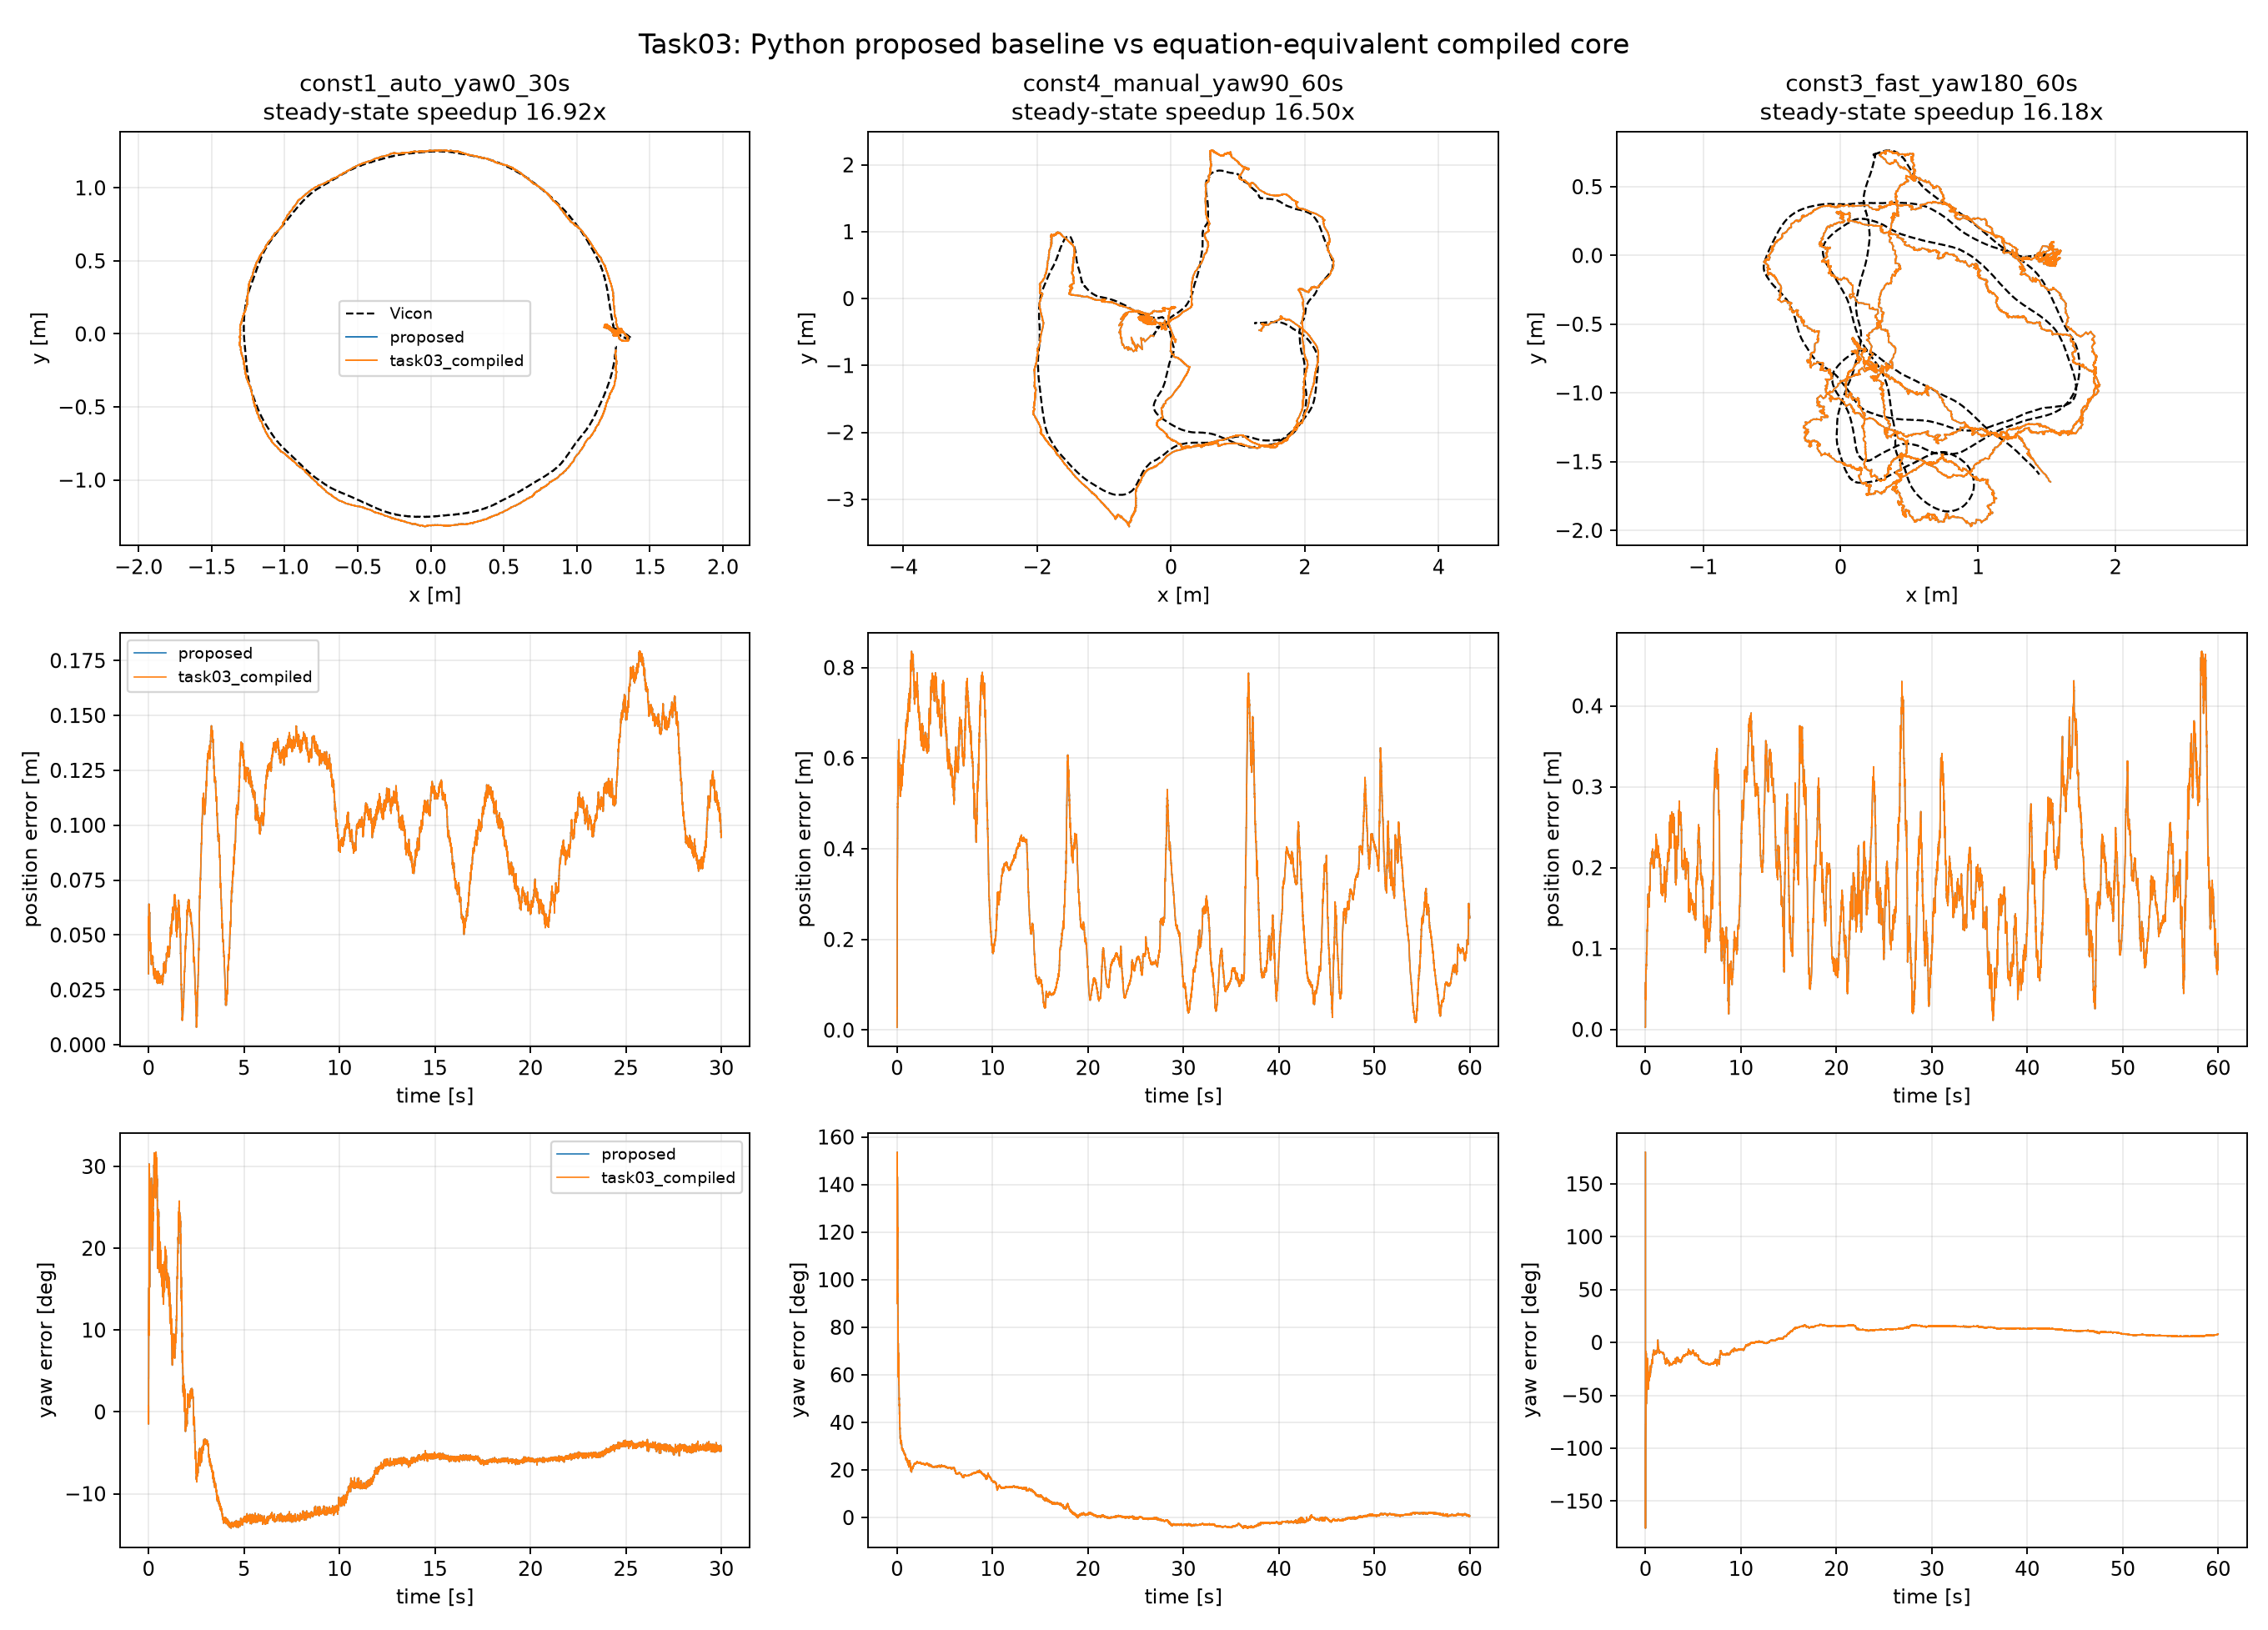
\includegraphics[width=\textwidth]{../imu-uwb-inekf/results/task03_compiled_optimization/comparison.png}
\caption{三组轨迹、位置误差与 yaw 误差。两种实现曲线重合；无新增跳变、发散或门限变化。}
\end{figure}

\section{边界与后续建议}

本结果证明的是 Windows 桌面、指定 Conda 环境、Numba 0.61.2 和
\texttt{float64} 下的稳定态离线回放。首次部署必须预热；Numba 缓存与 Python/
NumPy/CPU 绑定，环境升级后应重新编译。当前编译核是生产公式的独立实现，今后修改
Python \texttt{proposed} 方程时，必须同步修改并继续运行逐元素回归测试。

由于 60 s 数据已能在约 0.5 s 内完成，下一优先级应从“继续激进近似”转向目标硬件
WCET、内存和流式接口验证。只有目标硬件仍不满足预算时，才应逐项研究多速率或
12 维模式，并补充 NEES/NIS、IMU 降采样、温漂和模式恢复试验，而不能把理论算量
比例直接当成可交付加速。

\end{document}
